\documentclass{whiteboard}
\begin{document}
\begin{frame}[plain,t]
\bbcover{Programação Lógica}{Unificação}{Prof. Edson Alves}{Campus UnB Gama: Faculdade de Ciências e Tecnologias em Engenharia}

\end{frame}
\begin{frame}[plain,t]
\begin{tikzpicture}
\node[draw,opacity=0] at (0, 0) {x};
\node[draw,opacity=0] at (14, 8) {x};

	\node[anchor=west] (title) at (0.0, 7.0) { \Large \bbbold{Processos de unificação} };

\end{tikzpicture}
\end{frame}
\begin{frame}[plain,t]
\begin{tikzpicture}
\node[draw,opacity=0] at (0, 0) {x};
\node[draw,opacity=0] at (14, 8) {x};

	\node[anchor=west] (title) at (0.0, 7.0) { \Large \bbbold{Processos de unificação} };


	\draw[very thick] (0.0, 6.0) to  (13.5, 6.0);

	\draw[thick] (0.0, 5.0) to  (13.5, 5.0);

	\node[] (op) at (2.0, 5.5) { \bbemph{Elementos} };

	\node[anchor=west] (read) at (4.5, 5.5) { \bbemph{Comportamento} };

\end{tikzpicture}
\end{frame}
\begin{frame}[plain,t]
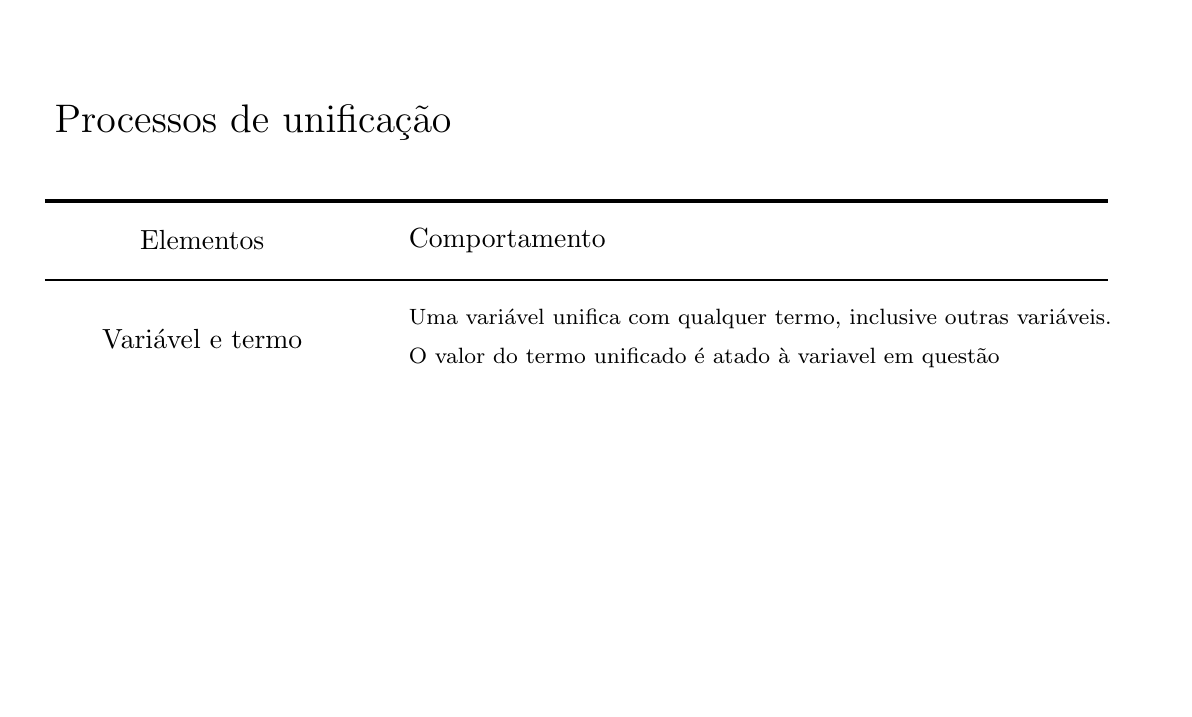
\begin{tikzpicture}
\node[draw,opacity=0] at (0, 0) {x};
\node[draw,opacity=0] at (14, 8) {x};

	\node[anchor=west] (title) at (0.0, 7.0) { \Large \bbbold{Processos de unificação} };


	\draw[very thick] (0.0, 6.0) to  (13.5, 6.0);

	\draw[thick] (0.0, 5.0) to  (13.5, 5.0);

	\node[] (op) at (2.0, 5.5) { \bbemph{Elementos} };

	\node[anchor=west] (read) at (4.5, 5.5) { \bbemph{Comportamento} };


	\node[] (not) at (2.0, 4.25) { \bbtext{Variável e termo} };

	\node[anchor=west] (not_read) at (4.5, 4.5) { \footnotesize \bbtext{Uma variável unifica com qualquer termo, inclusive outras variáveis. } };

	\node[anchor=west] (not_desc) at (4.5, 4.0) { \footnotesize \bbtext{O valor do termo unificado é atado à variavel em questão} };

\end{tikzpicture}
\end{frame}
\begin{frame}[plain,t]
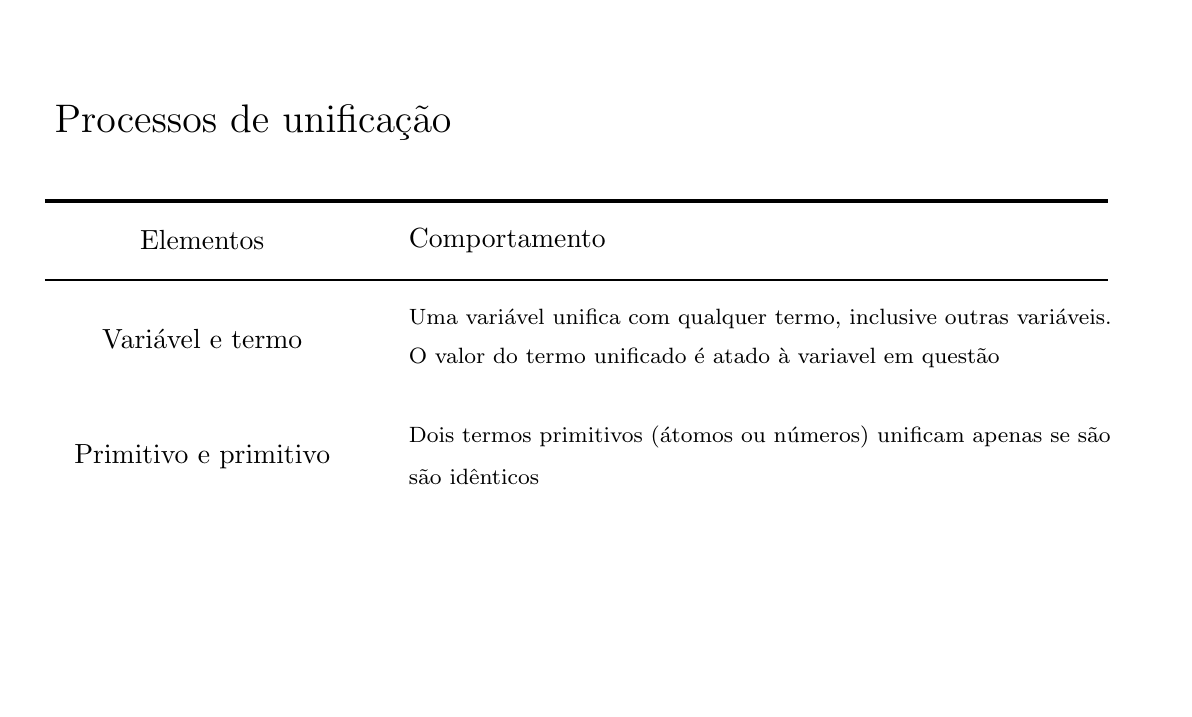
\begin{tikzpicture}
\node[draw,opacity=0] at (0, 0) {x};
\node[draw,opacity=0] at (14, 8) {x};

	\node[anchor=west] (title) at (0.0, 7.0) { \Large \bbbold{Processos de unificação} };


	\draw[very thick] (0.0, 6.0) to  (13.5, 6.0);

	\draw[thick] (0.0, 5.0) to  (13.5, 5.0);

	\node[] (op) at (2.0, 5.5) { \bbemph{Elementos} };

	\node[anchor=west] (read) at (4.5, 5.5) { \bbemph{Comportamento} };


	\node[] (not) at (2.0, 4.25) { \bbtext{Variável e termo} };

	\node[anchor=west] (not_read) at (4.5, 4.5) { \footnotesize \bbtext{Uma variável unifica com qualquer termo, inclusive outras variáveis. } };

	\node[anchor=west] (not_desc) at (4.5, 4.0) { \footnotesize \bbtext{O valor do termo unificado é atado à variavel em questão} };


	\node[] (or) at (2.0, 2.75) { \bbtext{Primitivo e primitivo} };

	\node[anchor=west] (or_read) at (4.5, 3.0) { \footnotesize \bbtext{Dois termos primitivos (átomos ou números) unificam apenas se são} };

	\node[anchor=west] (or_desc) at (4.5, 2.5) { \footnotesize \bbtext{são idênticos} };

\end{tikzpicture}
\end{frame}
\begin{frame}[plain,t]
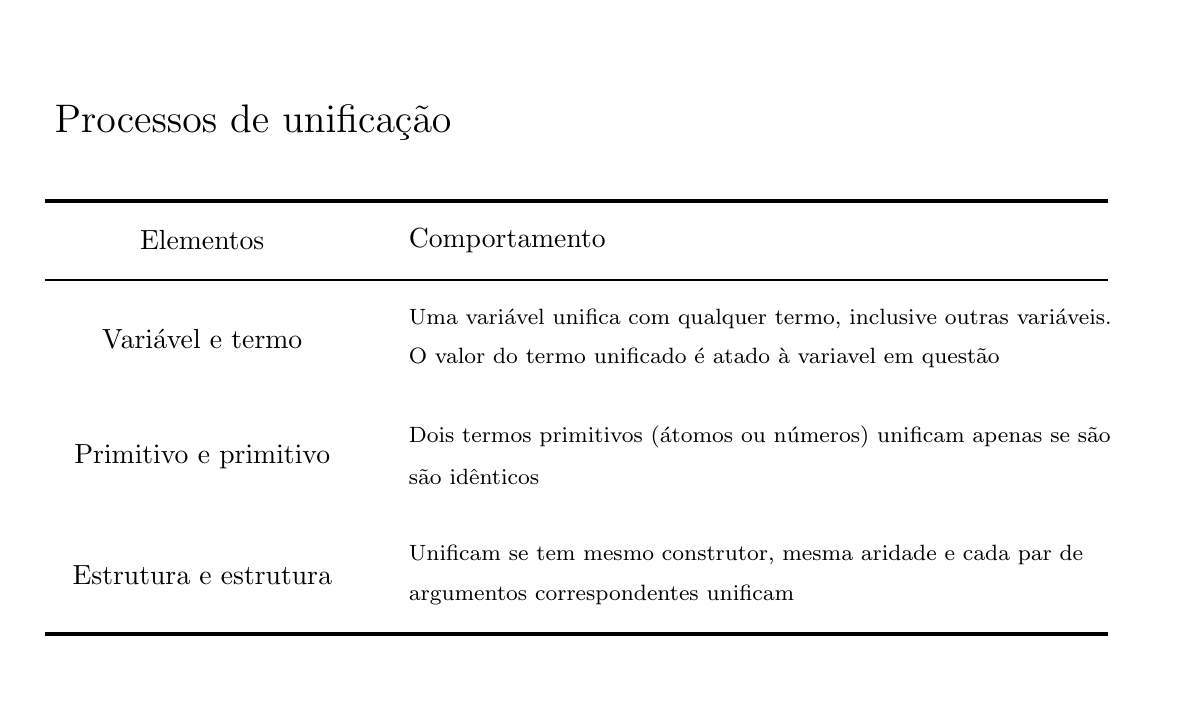
\begin{tikzpicture}
\node[draw,opacity=0] at (0, 0) {x};
\node[draw,opacity=0] at (14, 8) {x};

	\node[anchor=west] (title) at (0.0, 7.0) { \Large \bbbold{Processos de unificação} };


	\draw[very thick] (0.0, 6.0) to  (13.5, 6.0);

	\draw[thick] (0.0, 5.0) to  (13.5, 5.0);

	\node[] (op) at (2.0, 5.5) { \bbemph{Elementos} };

	\node[anchor=west] (read) at (4.5, 5.5) { \bbemph{Comportamento} };


	\node[] (not) at (2.0, 4.25) { \bbtext{Variável e termo} };

	\node[anchor=west] (not_read) at (4.5, 4.5) { \footnotesize \bbtext{Uma variável unifica com qualquer termo, inclusive outras variáveis. } };

	\node[anchor=west] (not_desc) at (4.5, 4.0) { \footnotesize \bbtext{O valor do termo unificado é atado à variavel em questão} };


	\node[] (or) at (2.0, 2.75) { \bbtext{Primitivo e primitivo} };

	\node[anchor=west] (or_read) at (4.5, 3.0) { \footnotesize \bbtext{Dois termos primitivos (átomos ou números) unificam apenas se são} };

	\node[anchor=west] (or_desc) at (4.5, 2.5) { \footnotesize \bbtext{são idênticos} };


	\node[] (and) at (2.0, 1.25) { \bbtext{Estrutura e estrutura} };

	\node[anchor=west] (and_read) at (4.5, 1.5) { \footnotesize \bbtext{Unificam se tem mesmo construtor, mesma aridade e cada par de} };

	\node[anchor=west] (and_desc) at (4.5, 1.0) { \footnotesize \bbtext{argumentos correspondentes unificam} };


	\draw[very thick] (0.0, 0.5) to  (13.5, 0.5);

\end{tikzpicture}
\end{frame}
\end{document}
